\documentclass[10pt]{beamer}

\usetheme{metropolis}
\usepackage{appendixnumberbeamer,amsmath}
\usepackage[ruled,vlined]{algorithm2e}
\usepackage{booktabs}
\usepackage[scale=2]{ccicons}
\usepackage{tikz}
\usetikzlibrary{arrows.meta,positioning,calc,decorations.pathreplacing}

\DeclareMathOperator{\order}{Order}

\usepackage{libertine}
\usepackage[libertine]{newtxmath}
\usepackage{mathrsfs}
\include{../../letterfonts}
\DeclareMathOperator{\enc}{Enc}
\DeclareMathOperator{\res}{Res}
\DeclareMathOperator{\spec}{Spec}
\DeclareMathOperator{\cov}{Cov}
\DeclareMathOperator{\Var}{Var}
\DeclareMathOperator{\Rank}{rank}
\newcommand{\Tfae}{The following are equivalent:}
\newcommand{\tfae}{the following are equivalent:}
\newcommand{\sparsity}{\textit{sparsity}}
\DeclareMathOperator{\poly}{poly}
\newtheorem{claim}{Claim}
\title{Nisan's Pseudorandom Generator for \textsf{RL}}
\subtitle{$\textsf{BPL}\subseteq \textsf{SC}=\textsf{DTISP}(\poly(n),\log^2(n))$}
\date{December 2, 2025}
\author{Soham Chatterjee}
\institute{Pesudorandomness Course (CSS.413.1) Presentation, STCS}
\metroset{block=fill}
\pagestyle{empty}
\begin{document}

\maketitle

% \begin{frame}{Table of contents}
% 	\setbeamertemplate{section in toc}[sections numbered]
% 	\tableofcontents[hideallsubsections]
% \end{frame}
\begin{frame}{Complexity Classes}
	\begin{itemize}
		\item \textsf{L}: Deterministic Logarithmic Space.
		\item $\mathsf{L}^\alpha$, $\alpha> 0$: Set of problems decidable in $O(\log^{\alpha}n)$ space deterministically.
		\item \textsf{NL}: Nondeterministic Logarithmic Space.
		\item \textsf{RL}: Randomized Logarithmic Space with One-sided error $\frac13$. 
		\item \textsf{BPL}: Randomized Logarithmic Space with Two-sided error $\frac13$.
		\item \textsf{SC}: Steve's Class or \textsf{DTISP}$(\poly(n),\poly(\log n))$ i.e. set of problems decidable deterministically in polynomial time and polylog space.
		\item \textsf{NC}: Nick's Class i.e. set of problems decidable in circuits of polynomial size and polylog depth and bounded fan-in. 
	\end{itemize}
	\begin{alertblock}{Remark}
		Don't confuse \textsf{SC} with $\mathsf{P}\cap \textsf{PolylogSpace}$!
	\end{alertblock}
\end{frame}
\begin{frame}[c]{Complexity Classes Zoo}

	\centering
	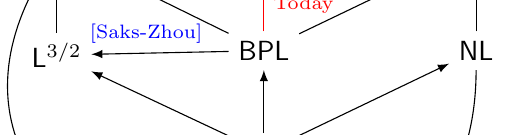
\begin{tikzpicture}[
			node distance=0.8cm and 2cm,
			class/.style={font=\sffamily},
			arrow/.style={-latex},
			annotation/.style={font=\scriptsize, text=blue}
		]
		\path[use as bounding box] (-3,-2) rectangle (3,-1);
		\node[class] (SC) at (0,0) {SC};
		\node[class, right=of SC] (NC) {NC};
		\node[class, left=of SC] (L2) {$\mathsf{L}^2$};

		% Now position other nodes relative to these
		\node[class, above=of NC] (P) {P};
		\node[class, above=of L2] (PolylogSpace) {PolylogSpace};
		\node[class, below=of SC] (BPL) {BPL};
		\node[class, below=of NC] (NL) {NL};
		\node[class, below=of L2] (L32) {$\mathsf{L}^{3/2}$};
		\node[class, below=of BPL] (RL) {RL};
		\node[class, below=of RL] (L) {L};

		% Draw arrows
		\draw[arrow] (L) -- (RL);
		\draw[arrow] (RL) -- (NL);
		\draw[arrow] (RL) -- (BPL);
		\draw[arrow] (RL) -- (L32);

		% From NL
		\draw[arrow] (NL) -- (NC);
		\draw[arrow] (NL) to[out=270,in=240,looseness=2.1] node[pos=0.7,annotation,above,sloped] {[Savitch]} (L2);

		% From BPL
		\draw[arrow] (BPL) -- (NC);
		\draw[arrow] (BPL) -- (L2);
		\draw[arrow] (BPL) -- node[midway,annotation,pos=0.6,above] {[Saks-Zhou]} (L32);

		% Left column
		\draw[arrow] (L32) -- (L2);
		\draw[arrow] (L2) -- (PolylogSpace);

		% From SC
		\draw[arrow] (SC) -- (PolylogSpace);
		\draw[arrow] (SC) -- (P);

		% From NC
		\draw[arrow] (NC) -- (P);
		% \draw[arrow, red] (BPL) -- node[midway,font=\scriptsize,right,pos=0.6,color=red] {Today} (SC);
		% \draw<1>[arrow] (BPL) -- (SC);

		% Red "Today" edge: appears starting slide 2
		\draw<2->[arrow, red] (BPL) --
		node[midway,font=\scriptsize,right,pos=0.6,color=red,align=left] {[Nisan]\\ Today} (SC);
	\end{tikzpicture}
\end{frame}
\begin{frame}{Pseudorandom Generator}
	\begin{definition}[Pseudorandom Generator]
		A map $\mcG:\{0,1\}^l\to \{0,1\}^n$, where $n\geq l$ is called a PRG for a class $\mcC$ with a parameter $\epsilon>0$ if for any $f\in \mcC$, $$\left|\underset{y\in\{0,1\}^n}{\bbP}[f(y)=1]-\underset{x\in\{0,1\}^l}{\bbP}[f(\mcG(x))=1]\right|\leq \epsilon$$
	\end{definition}
	\begin{itemize}
		\item Here $l$ is called the seed-length of the PRG.
		\item $n-l$ is called the stretch of the PRG.\pause
		\item We call $\mcG$, $\epsilon$-fools $\mcC$.\pause
		\item Typically, we want $n>> l$ and $\mcG$ to be efficiently computable.
	\end{itemize}
\end{frame}
\begin{frame}{Finite State Automata}
	Let $T$ be a \textsf{BPL} machine which uses $n^c$ random bits on inputs of length $n$ and runs in polynomial time and uses $S=O(\log n)$ space. \pause
	\begin{itemize}
		\item There are at most  $N:=2^{O(S)}=\poly(n)$ configurations of $T$. \pause
		\item Each random bit is used to make a transition between two configurations. \pause
		\item The starting configuration is fixed for any input. \pause
		\item Input $x$ is accepted if $T$ reaches a state representing acceptance.
	\end{itemize} \pause

	Therefore the configuration graph of $T$ on input $x$ represents a finite state automata with $N$ states.
\end{frame}
\begin{frame}[c]{Computational Tableau of \textsf{BPL} machine}
	\begin{figure}
		\centering
		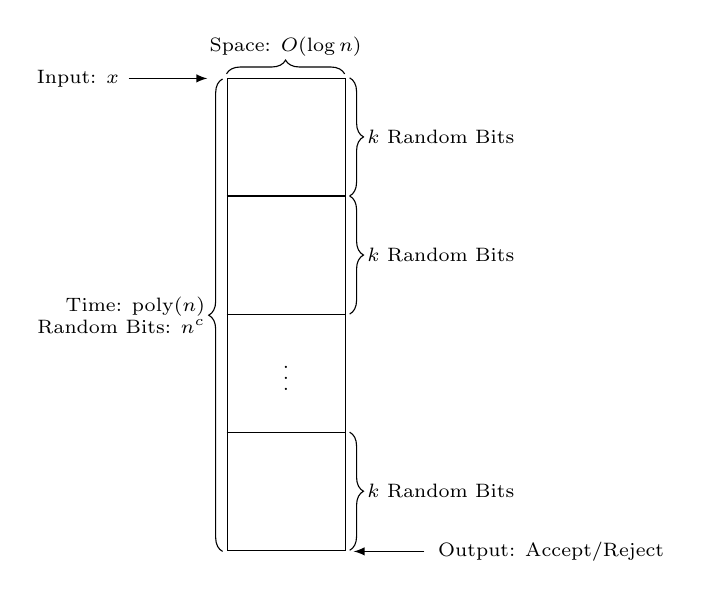
\begin{tikzpicture}[
				box/.style={draw, minimum width=1.5cm, minimum height=6cm},
				brace/.style={decorate,decoration={brace,amplitude=5pt}},
				arrow/.style={-latex},
				txt/.style={font=\scriptsize}
			]

			% Main box
			\node[box] (B) at (0,0) {};

			% Horizontal slices
			\draw (B.north west)++(0,-1.5) -- ++(1.5,0);
			\draw (B.north west)++(0,-3) -- ++(1.5,0);
			\draw (B.north west)++(0,-4.5) -- ++(1.5,0);

			% Left input arrow
			\draw[arrow] (-2,3) -- ++(+1,0);
			\node[txt, anchor=east] at (-2,3) {$\text{Input: } x$};

			% Right braces + text
			\draw[brace] (B.north east)++(+0.05,0) -- ++(0,-1.5)
			node[midway,right=0.1cm,txt] {$k$ Random Bits};

			\draw[brace] (B.north east)++(+0.05,-1.5) -- ++(0,-1.5)
			node[midway,right=0.1cm,txt] {$k$ Random Bits};

			\draw[brace] (B.north east)++(+0.05,-4.5) -- ++(0,-1.5)
			node[midway,right=0.1cm,txt] {$k$ Random Bits};
			% Left Brace + text
			\draw[brace]
			(B.south west)++(-0.05,0) -- ++(0,6)
			node[midway, txt, left=0.1cm, align=right]{Time: $\poly(n)$\\ Random Bits: $n^{c}$};
			% Top Brace + text
			\draw[brace] (B.north west) ++(0,0.05) -- node[txt,midway,above=0.1cm] {Space: $ O(\log n)$}++(+1.5,0);
			% Bottom output arrow
			\draw[arrow] (B.south east) ++ (+1,0) node[txt,right=0.05cm,align=left] {Output: Accept/Reject} -- ++(-0.9,0);

			% Annotations
			\node[txt] at (0,-0.7) {$\vdots$};
		\end{tikzpicture}
		\caption{Computational Tableau of \textsf{BPL} machine $T$.}
	\end{figure}

\end{frame}
\begin{frame}{Dividing \textsf{BPL} Computation into Blocks}
	\begin{itemize}
		\item Let the \textsf{BPL} machine $T$ run in time $\poly(n)$ using $n^{c}$ random bits and $O(\log n)$ space on input $x$ of length $n$.\pause
		\item Let $k<< n^{c}$ be a parameter to be fixed later.
		\item Divide the computation of $T$ into $t=n^c/k$ blocks, where each block uses $k$ random bits.\pause
		\item We can treat each block as a separate \textsf{BPL} machine $T_i$ (in some sense) which takes input as the final configuration of $T_{i-1}$ and $k$ random bits.
	\end{itemize}
\end{frame}
\begin{frame}{FSA for Computation Blocks}
	\begin{itemize}
		\item We can think of $T$ as a finite state automata with $N$ states.
		\item Each state makes $2^k$ transitions where each transion corresponds to a choice of $k$ random bits. \pause
		\item Let $Q$ be this automata. For transition we write $Q(i;r)=j$ for any $r\in\{0,1\}^k$ if $Q$ goes from state $i$ to state $j$ when fed $r$. \pause
		\item Let $M$ be the matrix where $M[i,j]=\underset{r\in\{0,1\}^k}{\bbP}[Q(i;x)=j]$\pause
	\end{itemize}
	$$\underset{r\in \{0,1\}^{k\times t}}{\bbP}[T(x,r)=\text{Acc}]=\sum_{j:\text{Accepting state}}M^t[1,j]$$

	\textbf{Goal:} Approximate $M^t$ using PRG.
\end{frame}
\begin{frame}{Approximate Automata Matrix}
	Suppose we have a pseudorandom generator $\mcG:\{0,1\}^k\to \{0,1\}^{k\cdot t}$. Let $Q$ be a finite state automata with $N$ states and its matrix be $M$ as defined above.\pause
	\begin{itemize}
		\item From definition of $M$, $M^t[i,j]=\underset{r_1,\dots, r_t\in\{0,1\}^k}{\bbP}[Q(i;r_1\dots ;r_t)=j]$\pause
		\item Using $\mcG$, let $M_{\mcG}[i,j]=\underset{r\in\{0,1\}^k}{\bbP}[Q(i;\mcG(r))=j]$\pause
		\item Want to construct $\mcG$ such that $$\|M^t-M_{\mcG}\|<\epsilon$$ for small $\epsilon$.
	\end{itemize} \pause
	Then if $T$ decides a language with error probability at most $\frac13$, using $\mcG$ we can calculate the $\sum_{j:\text{Accepting state}}M_{\mcG}[1,j]$ and decide the language if  it is at least $\frac23-\epsilon$.
\end{frame}
\begin{frame}{Matrix Norm}
	For any vector $v\in \bbR^N$, define $\|v\|=\sum_{i\in [N]}|v(i)|$. Then for any matrix $M\in \bbR^{N\times N}$ define $$\|M\|=\sup\limits_{0\neq v\in\bbR^N}\frac{\|Mv\|}{\|v\|}$$

	\textbf{Properties:}\begin{itemize}
		\item $\|M\|\leq\max\limits_{i\in [N]}\sum_{j\in [N]}|M[i,j]|$
		\item $\|M+N\|\leq \|M\|+\|N\|$
		\item $\|MN\|\leq \|M\|\cdot \|N\|$
	\end{itemize}
\end{frame}
\begin{frame}{Universal Hash Family}
	\begin{definition}[Universal Hash Family (Carter-Wegman)]
		$\mcH=\{h:\{0,1\}^k\to\{0,1\}^m\}$ is a \textit{universal hash family} if for any $x_1\neq x_2\in\{0,1\}^k$ and $y_1,y_2\in\{0,1\}^m$,\begin{itemize}
			\item $\underset{h \in \mathcal{H}}{\bbP}[\,h(x_1) = y_1\,] \;=\; \frac{1}{2^m}$
			\item $\underset{h \in \mathcal{H}}{\bbP}[\,h(x_1)=y_1 \;\wedge\; h(x_2)=y_2\,]
				      \;=\; \frac{1}{2^{2m}}$
		\end{itemize}
	\end{definition}\pause

	\vfill

	\begin{itemize}
		\item For our purpose, we have $k=m$. \pause
		\item We can construct such a family with $|\mcH|=2^{O(k)}$ where $$\mcH=\{a\cdot x+ b\mid a,b\in\{0,1\}^k\}$$ over $GF(2^k)$.
	\end{itemize}
\end{frame}
\begin{frame}{Property of Universal Hash Family}
	\begin{definition}[$(\epsilon,A,B)$-good hash function]
		Let $A\subseteq \{0,1\}^k$, $B\subseteq \{0,1\}^m$, $\epsilon>0$, $h:\{0,1\}^k\to\{0,1\}^m$ is said to be \textit{$(\epsilon,A,B)$-good} if
		$$\left|\underset{x\in\{0,1\}^k}{\bbP}[x\in A\wedge h(x)\in B]-\alpha\cdot \beta\right|\leq \epsilon$$
		where $\alpha=\frac{|A|}{2^k}$ and $\beta=\frac{|B|}{2^m}$.
	\end{definition}\pause

	\vfill

	\begin{lemma}[Proved in Appendix]
		If $\mcH$ is a universal hash family, then for any $A\subseteq \{0,1\}^k$, $B\subseteq \{0,1\}^m$, $\epsilon>0$, $$\underset{h\in\mcH}{\bbP}[h\text{ is not $(\epsilon,A,B)$-good}]\leq \frac{\alpha\cdot\beta}{2^k\epsilon^2}$$
	\end{lemma}

	% For $k=m$, by union bound an uniformly random $h$ is $\left(\frac{\epsilon}{k^2}, A,B\right)$-good for all $A,B$.
\end{frame}
\begin{frame}{Nisan's Generator}
	Let $\mcH$ be an universal hash family from $\{0,1\}^k$ to $\{0,1\}^k$. For any integer $m\geq 0$ define the function $\mcG_m\colon\{0,1\}^k\times \mcH^{m}\to \{0,1\}^{k\cdot 2^m}$ recursively as follows:\pause
	\begin{itemize}
		\item $\mcG_0(x)=x$
		\item $\mcG_m(x,h_1,\dots, h_m)=(\mcG_{m-1}(x,h_1,\dots ,h_{m-1}), \mcG_{m-1}(h_m(x),h_1,\dots, h_{m-1}))$
	\end{itemize}\pause

	For example: $$\mcG_1(x,h)=(x,h(x)),\quad \mcG_2(x,h_1,h_2)=(x,h_1(x), h_2(x), h_1\cdot h_2(x))$$ \pause
	$$\mcG_3(x,h_1,h_2,h_3)=(x,h_1(x), h_2(x), h_1\cdot h_2(x), h_3(x), h_1\cdot h_3(x), h_2\cdot h_3(x), h_1\cdot h_2\cdot h_3(x))$$\pause

	\begin{itemize}
		\item We want $k\cdot 2^m=n^c\implies m=\log t$.
		\item This gives a stretch of $k\cdot (t-1)$ bits.
	\end{itemize}
\end{frame}
\begin{frame}{Proof Flow}
	Let $h_1,\dots, h_s$ be some fixed hash functions from $\mcH$.  Define the matrix $$M_{h_1,\dots, h_s}[i,j]=\underset{x\in\{0,1\}^k}{\bbP}[Q(i;\mcG_s(x,h_1,\dots, h_s))=j]$$
	\vspace{-0.5cm}

	\begin{itemize}
		\item Using $h_1,\dots, h_s$ we had $2^s$ many transitions in $Q$. So we should compare $M_{h_1,\dots, h_s}$ with $M^{2^s}$.
	\end{itemize}\pause

	\textbf{Goal:} For `good' choice of $h_1,\dots, h_m$, $\|M^{2^m}-M_{h_1,\dots, h_m}\|<\epsilon$\pause

	\textbf{Approach:}

	\textbf{Step 1:} Suppose we have $h_1,\dots, h_{s-1}$. We will find $h_s\in \mcH$ such that for all $i,j\in [N]$, $$\left\|M^2_{h_1,\dots, h_{s-1}}-M_{h_1,\dots, h_s}\right\|\leq \delta$$\pause
	\textbf{Step 2:} Using above property will show for all $s\in[m]$, $$\left\|M_{h_1,\dots, h_s}-M^{2^s}\right\|\leq (2^s-1)\delta$$
\end{frame}
\begin{frame}{Find good $h_s$ from $h_1,\dots, h_{s-1}$}
	Suppose we have $h_1,\dots, h_{s-1}\in \mcH$ such that, $$ \left\|M_{h_1,\dots, h_{ls-1}}-M^{2^{s-1}}\right\|\leq (2^{s-1}-1)\delta$$If we can find $h_s$ such that $\|M^2_{h_1,\dots, h_{s-1}}-M_{h_1,\dots, h_s}\|\leq \delta$ then we are done.\pause

	\textbf{Algorithm (\textsc{Find}):} Go over all $h\in \mcH$ and all $i,j\in [N]$:\pause

	\textbf{Step 1:}  Compute \begin{itemize}
		\item $p_1=M_{h_1,\dots, h_{s-1}, h}[i,j]$
		\item $p_{2}=\sum_{l\in [N]}M_{h_1,\dots, h_{s-1}}[i,l]\cdot M_{h_1,\dots, h_{s-1}}[l,j]$
	\end{itemize}\pause
	\textbf{Step 2:} Check if $|p_1-p_2|>\frac{\delta}{N}$ go to next $h$ else return $h$.\pause
\begin{alertblock}{Remark}
	To compute $M_{h_1,\dots, h_{s-1}, h}[i,j]$ it goes over all $r\in\{0,1\}^k$ and compute $\mcG_s(r;h)1,\dots, h_s)$ and counts how many $r$ gives $Q(i;\mcG_s(r,h_1,\dots, h_s))=j$. and return $count/2^k$.
\end{alertblock}
	% To compute $M_{h_1,\dots, h_{s}}[i,j]$, go over all $r\in\{0,1\}^k$ and count how many $r$ gives, $Q(i;\mcG_s(r,h_1,\dots, h_s))=j$. then return $count/2^k$.

\end{frame}
\begin{frame}{Algorithm always returns an $h$\hfill (I)}
	\begin{claim}
		There exists an $h_s\in\mcH$ such that for all $i,j\in [N]$, $$\left|M_{h_1,\dots, h_{s-1}, h_s}[i,j]-M_{h_1,\dots, h_{s-1}}^2[i,j]\right|\leq \frac{\delta}{N}$$
	\end{claim}\pause
	Let $A_{i,j}$ be the set of $r\in\{0,1\}^k$ such that $Q(i;\mcG_{s-1}(r,h_1,\dots, h_{s-1}))=j$. So $M_{h_1,\dots, h_{s-1}}[i,j]=\rho(A_{i,j})$ where $\rho(A)=|A|/2^k$.\pause


	\begin{itemize}
		\item For any $i,j\in[N]$, $$M^2_{h_1,\dots, h_{s-1}}=\sum_{l\in[N]}\rho(A_{i,l})\cdot \rho(A_{l,j})$$\pause
		\item For any $h\in\mcH$, $$M_{h_1,\dots, h_{s-1}, h}[i,j]=\sum_{l\in[N]}\underset{r\in\{0,1\}^k}{\bbP}[r\in A_{i,l}\wedge h(r)\in A_{l,j}]$$
	\end{itemize}

\end{frame}
\begin{frame}{Algorithm always returns an $h$ \hfill (II)}


	For a random $h\in\mcH$ with probability at least $1-\frac{N^4}{2^k\delta^2}\geq 1-\frac1{2n^3}$, $$\left|\underset{r\in\{0,1\}^k}{\bbP}[r\in A_{i,l}\wedge h(r)\in A_{l,j}]-\rho(A_{i,l})\cdot \rho(A_{l,j})\right|\leq \frac{\rho(A_{i,l})\cdot \rho(A_{l,j})}{k^2}\leq \frac{\delta}{N^2}$$\pause

	So by Union Bound random $h\in \mcH$, $(\frac{\dl}{N^2},A,B)$-good for all $A,B$ with probability at least $\frac12$.\pause

	\begin{align*}
		     & \left|M^2_{h_1,\dots, h_{s-1}}[i,j]- M_{h_1,\dots, h_{s-1}, h}[i,j]\right|                                                          \\
		\leq & \sum_{l\in[N]}\left|\underset{r\in\{0,1\}^k}{\bbP}[r\in A_{i,l}\wedge h(r)\in A_{l,j}]-\rho(A_{i,l})\cdot \rho(A_{l,j})\right| \\
		\leq &\; N^2\cdot \frac{\delta}{N^2}=\delta
	\end{align*}
\end{frame}
\begin{frame}{Algorithm returns \emph{good} $h_s$}
	\begin{claim}
		If $h_s$ is returned by the above algorithm, then $$\left\|M_{h_1,\dots, h_s}-M^{2^s}\right\|\leq (2^s-1)\delta$$\pause
	\end{claim}
	We have $\|M^2_{h_1,\dots, h_{s-1}}-M_{h_1,\dots, h_s}\|\leq \delta$. \pause
	$$
		\|M_{h_1,\dots, h_s}-M^{2^s}\|  \leq \|M_{h_1,\dots, h_s}-M_{h_1,\dots, h_{s-1}}^2\|+\|M_{h_1,\dots, h_{s-1}}^2-M^{2^s}\|
	$$\pause
	\begin{align*}
		\|M_{h_1,\dots, h_{s-1}}^2-M^{2^s}\|
		 & \leq \|M_{h_1,\dots, h_{s-1}}\|\cdot \|M_{h_1,\dots, h_{s-1}}-M^{2^{s-1}}\|     \\
		 & \qquad \qquad\quad+ \|M_{h_1,\dots, h_{s-1}}-M^{2^{s-1}}\|\cdot \|M^{2^{s-1}}\| \\
		\uncover<5->{%
		 & \le 1\cdot (2^{s-1}-1)\delta
			+(2^{s-1}-1)\delta\cdot 1
			=(2^s-2)\delta
		}
	\end{align*}


\end{frame}
\begin{frame}{Setting Parameters}
	\begin{itemize}
		\item Set $k=\log(N)=O(\log n)$. So $t\approx n^c$.
	 \vfill 

		\item Set $m=\log t=O(\log n)$.
	 \vfill 
	 
		\item Want $(2^m-1)\delta=\epsilon\implies \delta=\frac{\epsilon}{2^m}$
	\end{itemize}
\end{frame}
\begin{frame}{Final Algorithm}
\begin{itemize}
	\item Compute $h_1,\dots, h_m$ one by one using the algorithm \textsc{Find}. \pause
	\item Compute $A[i,j]=M_{h_1,\dots, h_m}[i,j]$ for all $i,j\in[N]$. \pause
	\item Compute $\sum_{j:\text{Accepting state}}A[1,j]$ and accept if this is at least $\frac23-\epsilon$ else reject. 
\end{itemize}\pause
\textbf{Space:} The only place where more than $O(\log n)$ space is needed is to store the value of $h_1,\dots, h_m$. And each $h_i$ can be stored in $O(k)=O(\log n)$ space. So total space used is $O(\log^2 n)$. \pause

\textbf{Time:} For all $s\in[m]$, computing $M_{h_1,\dots, h_s}[i,j]$ takes $O(2^{k})$ times computation of $\mcG_s(r,h_1,\dots, h_s)$ for all $r$ and to check if $Q(i;\mcG_s(r,h_1,\dots, h_s))=j$ which takes $O(2^m)\cdot \poly(m)$ time. So \textsc{Find} takes $O(N^2\cdot 2^{2m}\cdot 2^{m+k})\poly(m)$. Hence total time $O(N^2\cdot 2^{2m}\cdot 2^{m+k})\poly(m)\cdot m=\poly(n)$. 
\end{frame}
\begin{frame}[standout]
	Thank You
\end{frame}
\begin{frame}[allowframebreaks]{Appendix}
	\begin{lemma}
		If $\mcH$ is a universal hash family, then for any $A\subseteq \{0,1\}^k$, $B\subseteq \{0,1\}^m$, $\epsilon>0$, $$\underset{h\in\mcH}{\bbP}[h\text{ is not $(\epsilon,A,B)$-good}]\leq \frac{\alpha\beta(1-\beta)}{2^k\epsilon^2}$$
	\end{lemma}
	

	Consider the matrix $M\in \{0,1\}^{2^k\times |\mcH|}$ where $M[x,h]=1$ if $h(x)\in B$ and $0$ otherwise. For any $x_1\neq x_2\in\{0,1\}^k$, $\underset{h\in\mcH}{\bbE}[M[x_1,h]]=\beta$ and  $ \underset{h\in\mcH}{\bbE}[M[x_1,h]M[x_2,h]]=\beta^2$

	\begin{align*}
		 \underset{h\in\mcH}{\bbE}\left[(\beta-\underset{x\in A}{\bbE}[M[x,h]])^2\right] & = \underset{x_1,x_2\in A}{\bbE}\ \underset{h\in\mcH}{\bbE}\left[(\beta-M[x_1,h])(\beta-M[x_2,h])\right]\\[-0.1cm]
		 & =  \underset{x_1,x_2\in A}{\bbE}\left[\beta^2-\beta \underset{h\in\mcH}{\bbE}[M[x_1,h]] -\beta\underset{h\in\mcH}{\bbE}[M[x_1,h]]\right.\\[-0.3cm]  
		 & \qquad\qquad\qquad\qquad\quad\; \left.+\underset{h\in\mcH}{\bbE}[M[x_1,h]\cdot M[x_2,h]]\right] \\[-0.2cm]
		  & = \underset{x_1,x_2\in A}{\bbE}\left[\underset{h\in\mcH}{\bbE}[M[x_1,h]\cdot M[x_2,h]]-\beta^2\right] 
	\end{align*}
\begin{itemize}
	\item For $x_1\neq x_2$: $\underset{h\in\mcH}{\bbE}[M[x_1,h]\cdot M[x_2,h]]=\beta^2$
	\item For $x_1=x_2$: $\underset{h\in\mcH}{\bbE}[M[x_1,h]\cdot M[x_2,h]]=\underset{h\in\mcH}{\bbE}[M[x_1,h]]=\beta$. 
\end{itemize} 

\framebreak
So,
$$\underset{h\in\mcH}{\bbE}\left[(\beta-\underset{x\in A}{\bbE}[M[x,h]])^2\right]=\frac1{|A|}(\beta-\beta^2)=\frac{\alpha\beta(1-\beta)}{2^k}$$


	Now $\underset{x\in \{0,1\}^k}{\bbP}[x\in A\wedge h(x)\in B]=\alpha\underset{x\in A}{\bbP}[h(x)\in B]=\alpha\cdot \underset{x\in A}{\bbE}[M[x,h]]$. So $h$ is not $(\epsilon,A,B)$-good iff $$\left|\underset{x\in A}{\bbE}[M[x,h]]-\beta\right|\geq \frac{\epsilon}{\alpha}$$

	By Markov, $$\underset{h\in\mcH}{\bbP}\left[\left|\beta-\underset{x\in A}{\bbE}[M[x,h]]\right|\geq \frac{\epsilon}{\alpha}\right]\leq \frac{\alpha\beta(1-\beta)}{2^k\epsilon^2}$$
\end{frame}
\end{document}
